\documentclass[10pt,a4paper]{article}

\usepackage[utf8]{inputenc}
\usepackage[T1]{fontenc}	
\usepackage[italian]{babel}
\usepackage{amsmath}
\usepackage{amsfonts}
\usepackage{amssymb}
\usepackage{graphicx}

\usepackage[left=2cm,right=2cm,top=2cm,bottom=2cm]{geometry}
\geometry{a4paper}

\usepackage{booktabs} % for much better looking tables
\usepackage{verbatim}
\usepackage{subfig} % make it possible to include more than one captioned figure/table in a single 

\usepackage{fancyhdr} % This should be set AFTER setting up the page geometry
\pagestyle{fancy} % options: empty , plain , fancy
\renewcommand{\headrulewidth}{0pt} % customise the layout...
\lhead{}\chead{}\rhead{}
\lfoot{}\cfoot{\thepage}\rfoot{}

%%% SECTION TITLE APPEARANCE
\usepackage{sectsty}
%\allsectionsfont{\sffamily\mdseries\upshape} % (See the fntguide.pdf for font help)
% (This matches ConTeXt defaults)
% pacchetti che mi fanno schifo ma uso lo stesso (Bob è scemo...)
\usepackage[cdot, thickqspace]{SIunits}
% macro che mi piacciono
\def\code#1{\texttt{#1}}


\title{Esercitazione 4: Amplificatore a transistor}

\author{Gruppo BE \\ Alessandro Candido, Roberto Ribatti}
\date{\today}
\begin{document}
\maketitle

\section{Scopo e strumentazione}
Lo scopo dell'esperienza è realizzare e caratterizzare un amplificatore a transistor, usando un transistor NPN 2N1711.

La strumentazione usata è quella presente sul banco di lavoro, più il suddetto transistor.

\section{Montaggio del circuito e punto di lavoro}
Il circuito è stato realizzato usando i componenti riportati in Tabella~\ref{tab:componenti}

\begin{table}[h!]
\centering
\begin{tabular}{c|c|c}
$R_1 = \unit{177.1 \pm 1.5}{\kilo\ohm}$ & $R_2 = \unit{18.06 \pm 0.15}{\kilo\ohm}$ & $R_C = \unit{9.93 \pm 0.09}{\kilo\ohm}$ & & $R_E = \unit{986 \pm 9}{\ohm}$ \\
$C_{IN} = \unit{230 \pm 10}{\nano\farad}$ & $C_{OUT} = \unit{98 \pm 6}{\nano\farad}$ & $C_E = \unit{100 \pm 10\%}{\micro\farad}$\\
\end{tabular}
\caption{Valori dei componenti utilizzati per la realizzazione dell'amplificatore}
\label{tab:componenti}
\end{table}

Ad eccezione dell'ultima parte dell'esperienza non è stata usata la resistenza $R_{es}$.

\subsection{Misure e valori attesi}

\paragraph{Punto di lavoro}
Si sono misurate corrente e tensione di quiescenza per determinare il punto di lavoro. Si riporta anche la tensione $V_{CC}$ erogata dall'alimentatore.
\begin{table}[h!]
\centering
\begin{tabular}{c|c|c}
$V_{CE}^Q = \unit{8.21 \pm 0.05}{\volt}$ & $I_C^Q = \unit{1.058 \pm 0.009}{\milli\ampere}$ & $V_{CC} = \unit{19.85 \pm 0.11}{\volt}$
\end{tabular}
\end{table}

Mentre i valori attesi sono\footnote{exp ad apice sta ad indicare che sono i valori attesi}:

\begin{table}[h!]
\centering
\begin{tabular}{c|c}
$V_{CE}^{exp} = \unit{8.03 \pm 0.23}{\volt}$ & $I_C^{exp} = \unit{1.082 \pm 0.022}{\milli\ampere}$
\end{tabular}
\end{table}

Per calcolarli si è usato che $V_{BE} = \unit{625 \pm 4}{\milli\volt}$, cioè quanto abbiamo misurato.

\paragraph{Tensioni ai terminali del transistor}
Le tensioni misurate sui terminali del transistor sono le seguenti.

\begin{table}[h!]
\centering
\begin{tabular}{c|c|c|c}
$V_B = \unit{1.692 \pm 0.009}{\volt}$ & $V_E = \unit{1.070 \pm 0.006}{\volt}$ & $V_{BE} = \unit{625 \pm 4}{\milli\volt}$ & $V_{C} = \unit{9.28 \pm 0.06}{\volt}$
\end{tabular}
\end{table}

Mentre per i valori attesi si è ottenuto:

\begin{table}[h!]
\centering
\begin{tabular}{c|c|c}
$V_B^{exp} = \unit{1.701 \pm 0.019}{\volt}$ & $V_E^{exp} = \unit{1.076 \pm 0.20}{\volt}$ & $V_{C}^{exp} = \unit{9.10 \pm 0.22}{\volt}$
\end{tabular}
\end{table}

%magari qui, e al punto precedente, dovrei mettere le formule usate, che alla fine sono quelle delle dispense

Non si riporta il valore atteso di $V_{BE}$ in quanto è stato usato proprio il valore misurato per ricavare gli altri. Si nota però che approssimativamente corrisponde ai valori tipici noti di $\sim \unit{0.6-0.7}{\volt}$
% non so se ha veramente senso includere quest'ultima parte

\paragraph{Compatibilità} Le misure sono tutte compatibili... %concludere leggendo da python

\subsection{Partitore $R_1-R_2$}
% scrivere Ib misurata (e attesa, ma forse non serve), confrontarla con I1 e I2 e concludere che non è stiff, ma prima di farlo rileggersi la definizione sulle dispense

\section{Risposta a segnali sinusoidali a frequenza fissa}
Si è misurato il guadagno per varie ampiezze del circuito amplificatore riportato sulla scheda, escludendo $C_E$ ed $R_E$ (cioè disconnettendoli).

\paragraph{Inversione di fase} Si è osservato che il segnale in uscita risultava in opposizione di fase rispetto al segnale in ingresso, come atteso. Si riporta in \figurename{\ref{fig:sfasamento}} la relativa schermata dell'oscilloscopio.

\begin{figure}[h!]
	\centering
	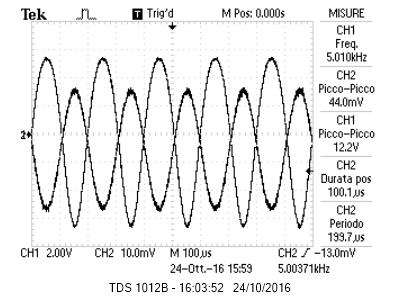
\includegraphics[width=0.54\textwidth]{../oscilloscopio/sfasamento.jpg}
	\caption{Sfasamento del segnale in uscita rispetto a quello in ingresso}
	\label{fig:sfasamento}
\end{figure}

\paragraph{Guadagno e linearità del circuito}
% fittare con una costante la parte fuori clipping, usare fitcostante di jack, e concludere

\paragraph{Clipping}
Il segnale in uscita risultava simmetrico fino ad ampiezze di $\sim \unit{1.7}{\volt}$ in ingresso.
% forse avremmo potuto stimare un errore su quei 1.7 V, magari possiamo stimarlo "a memoria"
Per intensità maggiori si osservava che l'uscita era tagliata dal basso. Questo taglio del segnale (riportato in \figurename{\ref{fig:clipping}}) corrisponde ad un regime di funzionamento del transistor diverso da quello attivo, in cui sarebbe preservata la linearità.

Si può identificare tale regime con quello di saturazione. Infatti quando scorre una maggiore corrente nel collettore si ha una caduta di potenziale maggiore su $R_C$, e dunque una minore tensione in uscita. Arrivando in saturazione il transistor non è in grado di erogare una corrente maggiore, e quindi la caduta di potenziale si assesta su un certo valore, finché la richiesta di corrente non diminuisce e il segnale in uscita riprende a salire.

\begin{figure}[h!]
	\centering
	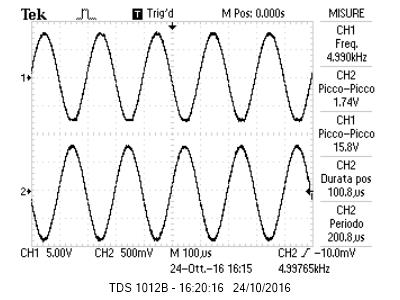
\includegraphics[width=0.54\textwidth]{../oscilloscopio/firstclipbasso.jpg}
	\caption{}
	\label{fig:clipping}
\end{figure}

Si era trovato che il punto di lavoro del transistor era fissato ad una corrente di collettore relativamente bassa, e quindi vicina al regime di interdizione. Tracciando la retta di carico si nota però che la pendenza di questa è relativamente piccola in valore assoluto, per cui, per ottenere spostamenti verticali\footnote{sul grafico delle curve caratteristiche di collettore, quindi piccole variazioni di $I_C$} anche ridotti, che porterebbero il transistor a lavorare in interdizione, si hanno notevoli spostamenti orizzontali\footnote{cioè variazioni di $V_{CE}$}, che portano dunque il transistor a lavorare in saturazione per segnali in ingresso di ampiezza minore rispetto a quelli che sarebbero necessari a portarlo in interdizione.
% poi ci metto qualche numerello per rendere la cosa più quantitativa

Per segnali in ingresso di ampiezza ancora maggiore ottengo il taglio dell'uscita anche dall'alto, arrivando a oscillare quindi tra i due regimi di saturazione e interdizione, si veda \figurename{\ref{fig:clippingdoppio}}

\begin{figure}[h!]
	\centering
	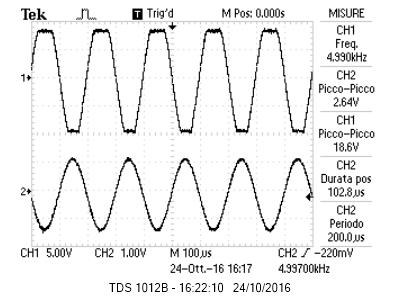
\includegraphics[width=0.54\textwidth]{../oscilloscopio/clipall.jpg}
	\caption{}
	\label{fig:clippingdoppio}
\end{figure}

\subsection{Impedenza d'ingresso}
% riportare le formule della scheda e scrivere quanto atteso e quanto misurato

\subsection{Impedenza d'uscita}
% come al punto precedente

\section{Risposta in frequenza}

\section{Aumento del guadagno}

\end{document}
